\documentclass[twocolumn]{article}
\usepackage[a4paper, top=2cm, bottom=2cm, left=1.5cm, right=1.5cm]{geometry}
\usepackage{float}        % <<< added for in place tables
\usepackage{graphicx}     % For including figures
\usepackage{amsmath}      % For math
\usepackage{booktabs}     % For nice tables
\usepackage{hyperref}     % For links
\usepackage{cite}         % For citations
\usepackage{pgfplots}     % <<< ADDED FOR PLOTTING
\pgfplotsset{compat=1.18} % <<< ADDED FOR PLOTTING

% CITATION: The figures in this report were created by me using a few youtube videos on latex and the AI assist on overleaf. After it did not show up correct I uploaded my current file to Gemini and asked for a bulleted list of changes to make the file compile correctly. (...it gave me the code for the correct formatted figures/tables)


\title{CS 431 Homework 01: Parallel Pi on OpenMP}
\author{David Haddad}
\date{\today}

\begin{document}

\maketitle

\section{Introduction}
This report details the implementation and performance analysis of two parallel algorithms for calculating $\pi$ using OpenMP. The first was the classic numerical integration method in which we calculated $4 \times (\textit{Area of $\frac{1}{4}$th circle)}$. The second (embarrassingly parallel) method was the Monte Carlo method in which we calculate the proportion of randomly generated points that lie within/without the circle.  The purpose of this assignment is to analyze the scalability and performance of these methods on the UO Talapas cluster. Throughout testing, the findings demonstrate key understandings of how synchronization strategies effect performance. The project itself illuminates the downsides of high-contention algorithms using a critical section and \texttt{atomic} and how that can actually cause negative speedup, while a \texttt{reduction}-based algorithm can achieve the expected linear speedup we want when scaling.  

\section{Methodology and Implementation}

All code for the project was written in C and parallelized using OpenMP. The initial serialized approach which was never taking longer than $4$s regardless of input size (up to $1B$). The theory was that the compiler was optimizing this code far past the current scope of the project. The \texttt{Makefile} compiler flags were altered from \texttt{-O3} (heavy optimizations) to the \texttt{-O0} flag (no optimization) to better demonstrate the true timing of the serialized approach as written in \texttt{pi.c}. However, the issue persisted. This "fake" baseline caused confusion and led to increasing the problem size to $100B$. Even this astronomically large input showed an unbelievable $~6$s for the serial approach. This meant that a $100x$ increase in size led to almost \textit{no change} in execution time. Since this could not be true, the final data set reduced the input size to $1B$ and we ignored the "serial baseline", instead focusing results on the correlations between the parallelized methods.

\subsection{P1: Parallel Integration with \texttt{atomic}}
This algorithm is the same as the serial method, with added OpenMP declarations. The use of the \texttt{\#pragma~omp~atomic} directive ensured that we avoided the race condition present without careful handling of the sum variable. This leads to serialization of this section of code, which creates a severe synchronization bottleneck.

\subsection{P2: Parallel Monte Carlo with \texttt{reduction}}
A common metaphor for this method is "dart throwing" in a loop and calculating the ratio of darts that "hit" and are \texttt{in\_circle} as $\pi$. This algorithm parallelizes that "dart-throwing" loop. Since each iteration of the loop is simply selection of a random point and checking if it's in the circle, they could all be run in parallel at the same time. However, this leads to a race condition and a similar bottleneck on the \texttt{in\_circle} variable if solved in the same way as \textbf{P1}. It was resolved using the OpenMP \texttt{reduction(+:in\_circle)} clause, giving each thread it's own copy and eliminating the bottleneck/unpredictable output.


\section{Results and Analysis}
The data collected illustrates how different synchronization strategies for the same underlying problem can have drastic differences in performance.

\subsection{Experimental Setup}

The data collected and used for the following figures was run using a series of \texttt{.srun} files and the following loop for data collection:
$$\texttt{for i in \{1..20\} do ./pi 1000000000 done } $$

Afterwards, the averages of the "$20$" runs were calculated.
Unfortunately, even with this input size, the Talapas cluster would cancel the jobs on the multi-threaded test scripts due to the \textbf{P1 Integration} method presenting negative performance scaling at a factor that caused the 4th or 5th iteration to reach the job \texttt{TIME LIMIT}.
Thus the averages calculated in the figures do not truly represent 20 runs for each method as that would require higher permissions/usage limit on Talapas.

\subsection{Analysis of P1 (Integration)}
The P1 algorithm demonstrated severe \textbf{negative scaling}. The baseline 1-thread time ($T_1$) was \textbf{6.817 seconds}. As shown in Table \ref{tab:p1_runtimes}, adding more threads ended up counter-productively and drastically \textit{increasing} the runtime.

\begin{table}[H]
  \centering
  \caption{P1 (\textit{atomic}) Performance vs. Thread Count}
  \label{tab:p1_runtimes} % Cite: had to look up how to use these I forgot
  \begin{tabular}{@{}ccc@{}} %???? Cite: got this is what gemini did to fix my formatting????
    \toprule % Cite: Youtube
    {Threads (p)} & {Avg. Time (s)} & {Speedup ($T_1/T_p$)}\\
    \midrule
    {1 (Baseline)}  &{6.817}& {1.00x}\\
    {2} & {45.863}  & {0.15x} \\
    {4} & {94.485}  & {0.07x} \\
    {8} & {128.712} & {0.05x}\\
    {16}& {121.172} & 0.06x \\
    \bottomrule
  \end{tabular}
\end{table}
These counterintuitive results are an example of \textit{high contention}. Instead of 16 threads running peacefully in parallel, the 16 threads end up waiting for access to the same \texttt{atomic} variable \textit{1 billion} times! The cost to synchronize and waiting completely surpass any benefit that came from increasing the number of threads. For some reason, the 16 threads ran faster than 8, but this was actually unique to the final data set as compared to the failed attempts (see output directory). Also, due to jobs being canceled before completing 20 iterations, random scheduling variance may account for this minor outlier.

\subsection{Analysis of P2 (Monte Carlo)}
To demonstrate the contrast, the project suggested the use of a \texttt{reduction} clause for this \textit{embarrassingly parallel} computation. In return, we see a almost perfect \textbf{linear~speedup}. The baseline time ($T_1$) was \textbf{12.466 seconds}. This result shows how using the correct OpenMP directives for the structure of your problem (and having an easy problem to parallelize) can successfully, and nearly completely, eliminate performance bottlenecks.

\begin{table}[H]
  \centering
  \caption{P2 (\textit{reduction}) Performance vs. Thread Count}
  \label{tab:p2_runtimes}
  \begin{tabular}{@{}ccc@{}}
    \toprule
    {Threads (p)}&{Avg. Time (s)} & {Speedup ($S_p$)}\\
    \midrule
    {1 (Baseline)} & {12.466} & {1.00x}\\
    {2} & {6.238} & {2.00x}\\
    {4} & {3.123} & {3.99x}\\
    {8} & {1.563} & {7.97x}\\
    {16}& {0.783} & {15.92x}\\
    \bottomrule
  \end{tabular}
\end{table}

Table \ref{tab:p2_runtimes} shows that as we doubled the threads, we consistently halved the runtime. These are the kind of consistent results that can be seen from successful and thoughtful parallelization of your code.

% --- THIS IS THE NEW FIGURE BLOCK ---
\begin{figure}[h!]
  \centering
  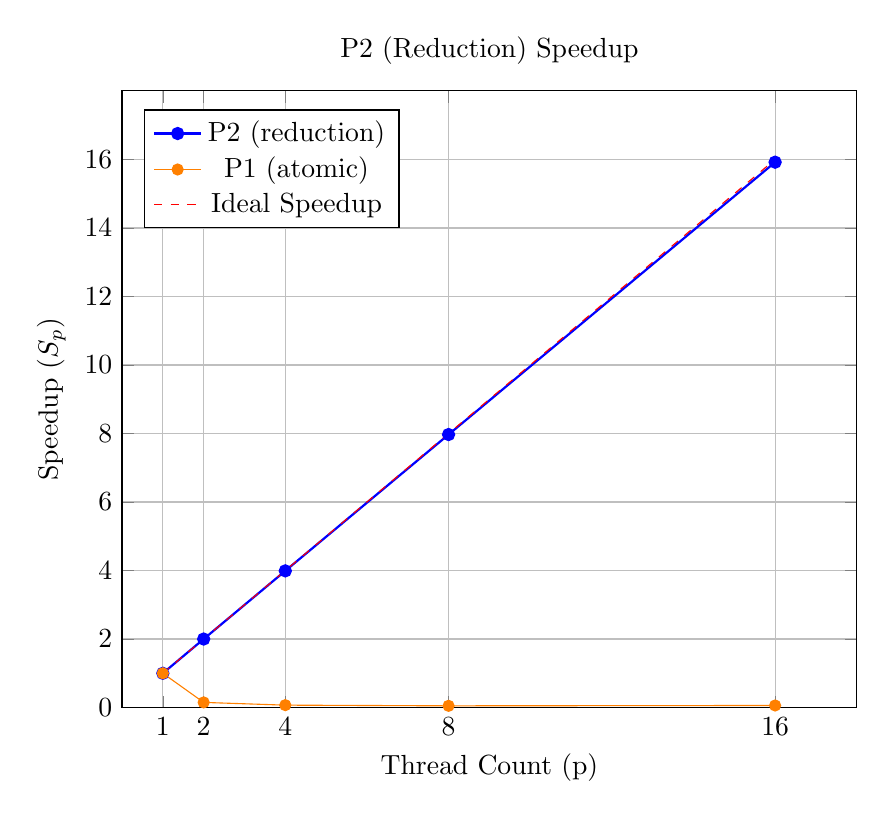
\begin{tikzpicture}
    \begin{axis}[
        title={P2 (Reduction) Speedup},
        xlabel={Thread Count (p)},
        ylabel={Speedup ($S_p$)},
        xmin=0, xmax=18,
        ymin=0, ymax=18,
        xtick={1, 2, 4, 8, 16},
        ytick={0, 2, 4, 6, 8, 10, 12, 14, 16},
        legend pos=north west,
        grid=major,
        width=0.9\columnwidth,
    ]
    
    % This is your P2 data from Table 2
    \addplot[
        color=blue,
        mark=*,
        thick,
    ]
    coordinates {
        (1, 1.00)
        (2, 2.00)
        (4, 3.99)
        (8, 7.97)
        (16, 15.92)
    };
    \addlegendentry{P2 (reduction)}

    % This is the P2 data from table 2. (i did this one on my own)
    \addplot[
        color=orange,
        mark=*,
        thin,
    ]
    coordinates {
        (1, 1.00 )
        (2, 0.15 )
        (4, 0.07 )
        (8, 0.05 )
        (16, 0.06 )
    };
    \addlegendentry{P1 (atomic)}
    
    % This is the "Ideal Speedup" y=x line
    \addplot[
        color=red,
        dashed,
        domain=1:16, % Plot from x=1 to x=16
    ]
    {x}; % The function y=x
    \addlegendentry{Ideal Speedup}

    \end{axis}
  \end{tikzpicture}
  \caption{Linear Speedup (red, dashed) vs Thread Count for P1 (atomic) and P2 (reduction). The P2's actual speedup (blue) almost perfectly the ideal linear speedup. P1's performance, however, decreased with increased thread count.}
  \label{fig:speedup}
\end{figure}
% END NEW AI GENERATED FIGURE BLOCK given data and \begin{figure} (MINE WOULD NOT SHOW UP!)
\end{document}